\documentclass{report}
\usepackage{textcomp}
\usepackage{mathtools}
\usepackage{enumitem}
\usepackage{cite}
\usepackage{titlesec}
\usepackage{graphicx}
\usepackage{float}
\usepackage[toc,page]{appendix}
\usepackage[margin=1in]{geometry}
\usepackage[doublespacing]{setspace}



\title{Physics BA Thesis}
\author{Christopher Don Milke}
\date{\today}


\graphicspath{ {images/} }

\titlespacing*{\chapter}{0pt}{0pt}{20pt}
\titleformat{\chapter}[display] {\normalfont\bfseries}{}{0pt}{\centering \LARGE}

\begin{document}
	\begin{titlepage}
        \maketitle
	\end{titlepage}

    \newpage
    \begin{center}
        \vspace*{\fill}
        Copyright \textcopyright by

        Christopher D. Milke 

        2016
        \vspace*{\fill}
    \end{center}
    \newpage

    \tableofcontents

    \chapter{ Background }
        \section{ The International Linear Collider }
            %in: None
            %out: Size of ILC, e+/- collider, collision energy, uses, ILC is precise b/c of parton distributions 
            \subsection{ What is the ILC and Why Does it Need to Exist? }
                \begin{figure}[h] 
                    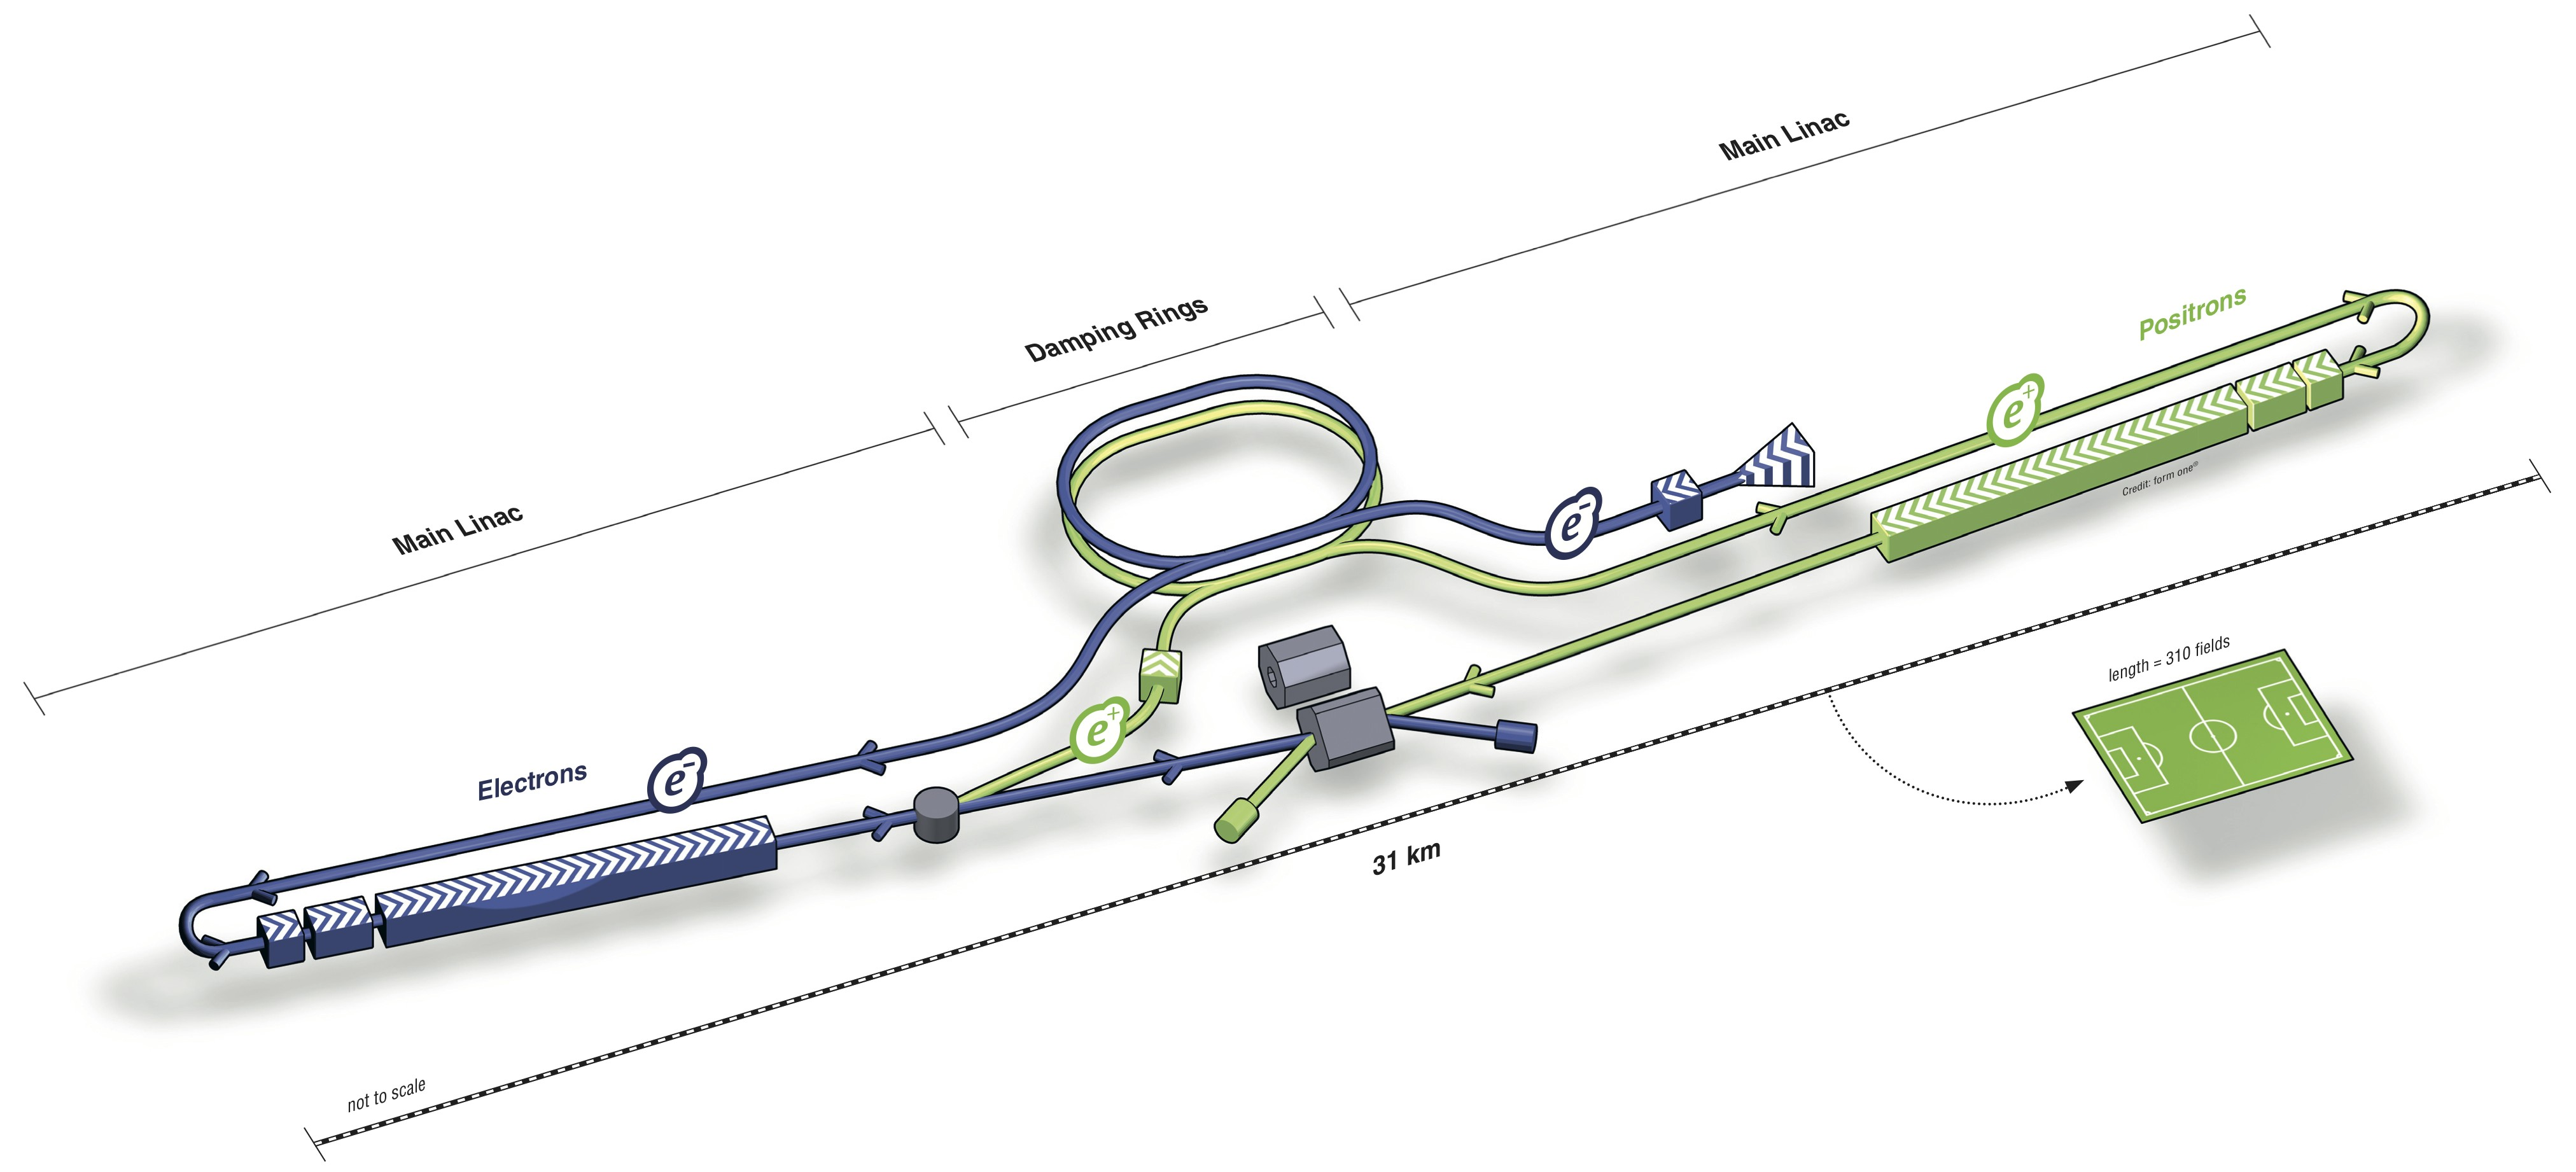
\includegraphics[width=\textwidth]{ilcoverview}
                    \centering
                    \caption{Overview of the ILC}
                    \label{fig:ilcoverview}
                \end{figure}

                The International Linear Collider (ILC) is a 30 kilometer long \cite{parton} linear particle accelerator \cite{specs} which will collide electrons and positrons together at 500 GeV energies. It will primarily be used for studying the properties of the Higgs Boson, attempting to find new dimensions, and trying to discover Supersymetric (SUSY) particles. All three of these are already being pursued by the much more powerful Large Hadron Collider (LHC), which begs the question of why the ILC is needed. The answer is that, while the LHC is significantly more powerful, the ILC will be significantly more precise. This is because the LHC is, as the name would imply, a hadron collider. In the simplest case, the LHC performs proton-proton collisions. However, protons are not elementary particles. They consist of three quarks and any number of gluons holding those quarks together. A collision between two protons then is actually a collision between six quarks and several gluons. This is a problem for physics studies in particle accelerators, because of something known as a parton distribution function. To understand why, a brief explanation of how one conducts particle accelerator physics studies is in order.

                All the physics processes mentioned, and indeed most other physics processes studied in particle colliders, are studied by reconstructing the paths and energies of particles as they traverse the various detector elements surrounding the particle collision point. The reconstructed paths are then compared to the initial state of the particles that went into the collision. The key statement here is that the comparison is to the particles' \textit{initial} state. While the positions and energies of the protons that are colliding may be well known, the same cannot be said for the individual quarks and gluons the proton is made up of. All that can be done for the constituent particles is to make estimates on where they \textit{might} be based a probabilistic distribution, known as a Parton Distribution Function (PDF). As a result, almost all studies done at the LHC (or any other hadron collider for that matter) face a constant source of significant systematic error on all results it produces. The ILC eliminates this issue entirely by colliding only electrons and positrons, both elementary particles that have no need of PDFs. As a result, the ILC can perform physics studies at a much more precise level, providing details on physics that the LHC cannot.

            %in: ILC context
            %out: tons of info on vertex and beamcal, albedo conflict, geom change list
            \subsection{An Overview of the Vertex Detector and BeamCal}
                \begin{figure}[h] 
                    \includegraphics[width=\textwidth]{sid_zoom1}
                    \centering
                    \caption{Zoomed in view of the SiD.
                        The Vertex Detector is circled in red,
                        the BeamCals in magenta.}
                    \label{fig:sid_zoom1}
                \end{figure}

                %in: What the ILC is
                %out: What is IP, what is SiD, size of SiD, location of Vertex and BeamCal,
                At the crossing of the positron and electron beams is the ILC's interaction point (IP). At any given time the IP can be surrounded by one of two exchangeable detectors: the Large International Detector (ILD) or the Silicon Detector (SiD). The focus in this study will be on the latter of the two. The SiD is an array of trackers and calorimeters over 12 meters long and over 16 meters in diameter. Of the numerous detectors it consists of, the two relevant to this study are the Vertex Detector and Beam Calorimeter (BeamCal). Both detectors are located extremely close to the IP of the SiD, in an area known as the Interaction Region (IR). 
                
                \begin{figure}[h]
                    \centering
                    \begin{minipage}{0.4\textwidth}
                        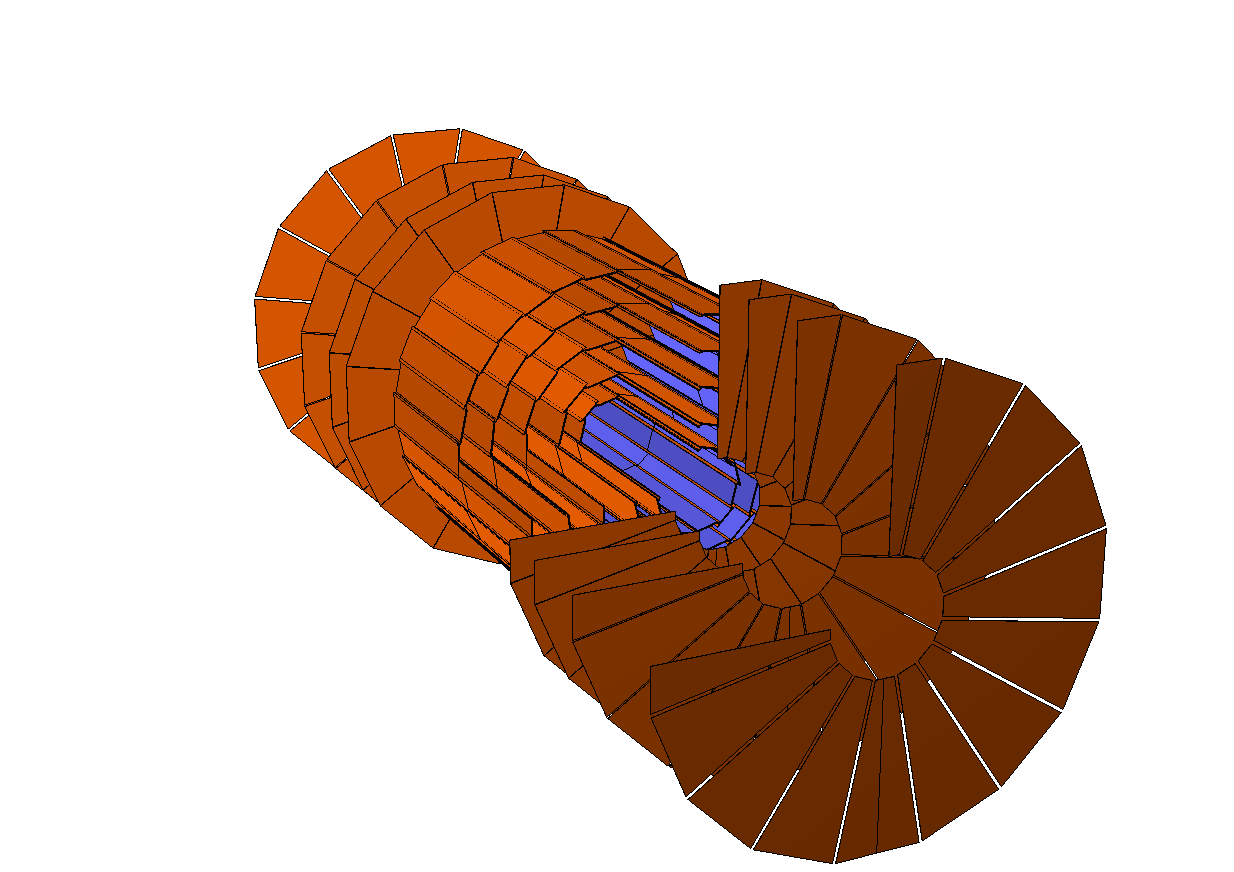
\includegraphics[width=\textwidth]{vertex}
                        \caption{Vertex Detector}
                        \label{fig:vertex}
                    \end{minipage}
                    \begin{minipage}{0.4\textwidth}
                        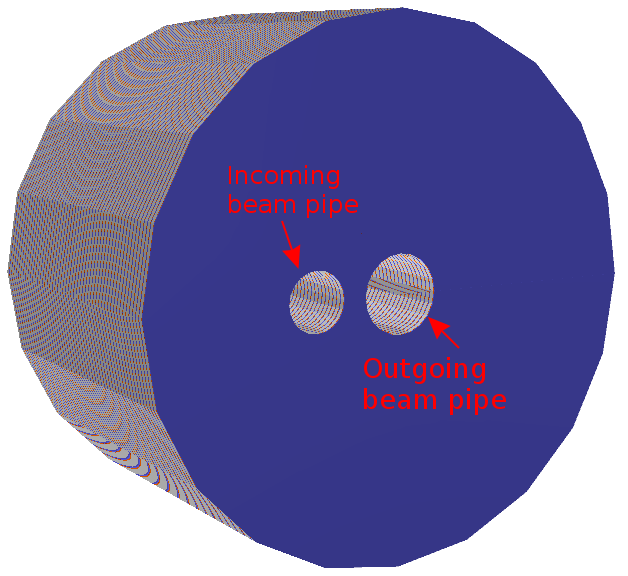
\includegraphics[width=\textwidth]{beamcal_full}
                        \caption{Beam Calorimeter}
                        \label{fig:beamcal}
                    \end{minipage}
                \end{figure}
                
                %in: context of vertex & beamcal 
                %out: location of Vertex and BeamCal, size of vertex, size of BeamCal, use of Vertex, advantages of vertex, beamcal only hit with lowpt particles, lowpt particles are often high energy, beamcal gets a lot of bgd energy, use of Vertex, advantages of vertex, beamcal only hit with lowpt particles, lowpt particles are often high energy, beamcal gets a lot of bgd energy
                The Vertex Detector, with a radius of only 6.3 centimeters and a length of 5.2 centimeters, immediately surrounds the IP. The BeamCal (or rather BeamCals, as the entire SiD is mirrored) is a fair distance away from the IP, at 32.65 meters. But with a radius of 14 centimeters, it closely hugs both the incoming and outgoing beam pipes, visible as holes in figure \ref{fig:beamcal}. The locations of the detectors provide unique advantages to each. For the Vertex Detector, surrounding the IP so closely means that it is often the first to detect particles, and, due its small size, is also able to use some of the most advanced electronics to perform this task. The BeamCal meanwhile sits in such a far away location, with such a small radius, that the only particles which hit it are those with extremely low transverse momenta. Generally the only particles with such a low trajectory angle are those which have had minimal interaction with other particles, and have thus retained most of their energy. As a result, the BeamCal is hit by some of the highest energy particles produced by the electron/positron collision. Aside from their near-beampipe locations though, the Vertex Detector and BeamCal function in almost diametrically opposed ways.

                %in: what vertex & beamcal are
                %out: how vertex works, importance of low vertex occupancy, how beamcal works, intro to albedo problem
                The Vertex Detector is a tracker-style detector, designed to track the positions of particles as they move through its layers. By identifying hits from a particle across the Vertex Detector's layers, the particle's trajectory can be determined. The Vertex Detector is built to interact with the particle as little as possible, so as not to interfere with the particle's trajectory. Moreover, it is critically important that the occupancy (the number of particles hitting the detector) be kept as low as possible. If the occupancy is too high, then it becomes difficult or impossible to effectively reconstruct particle trajectories. The BeamCal, on the other hand, is designed primarily for calorimetry, determining the energy of a particle (in addition to some minor position tracking). This is accomplished by interspersing silicon detector plates with large amounts of tungsten. The tungsten scatters and absorbs the energy of any particles hitting it, eventually stopping them completely. Energy is then measured by looking at how many layers of tungsten a particle was able to traverse before being stopped. This method of measuring energy is also the basis of a conflict between the Vertex Detector and BeamCal. Because the BeamCal effectively acts as a wall to all incoming particles, some of the particles actually ricochet backwards off of it, in an effect called \textit{albedo}. These showers of albedo particles rebounding off the BeamCal then proceed to fly back towards the IP, and into the Vertex Detector.
                
                %in: what is albedo, vertex, and beamcal
                %out: conflict between beamcal and vertex, list three changes
                The effect requires a careful balancing act. On one end of the scale, albedo increases the occupancy in the Vertex Detector, and should thus be kept to a minimum. On the other end, the BeamCal is a crucial component of the SiD, necessary for low transverse momentum particle tagging and beam parameter checking. The BeamCal cannot be removed, but its presence negatively effects the performance of the Vertex Detector. This study aims to research the effects of three independent changes to the architecture of the Interaction Region on this balance, analyzing how each of the changes alters the effectiveness of the Vertex Detector and BeamCal. The first change is with regard to the proximity of the BeamCal to the IP, the second studies the effects of cutting out part of the BeamCal, and the third determines the usefulness of a specialized magnetic field known as the anti-DiD.



        \section{Modifications to the SiD} \label{sect:sid_mods}
            %in: what is sid, IP, beamcal
            %out: what is L*, relavence to beamcal
            \subsection{L Star}

                The L* of the SiD is a term which refers to the distance between the Interaction Point and the beginning of the cryostat. The most recent technical design report for the SiD specified that for a number of reasons the cryostat needed to be be moved farther away from the Interaction Point, from 3.5 meters to 4.1 meters. The relevance of this change to detector studies is that the BeamCal is attached to the cryostat, so moving the cryostat also means moving the BeamCal (from 2.95 meters to 3.265 meters). This decision has already been made, and so the studies in the analysis section are only to see what the effect of this change is; the results of this study will not affect the design decision.


            %in: context of beamcal, albedo
            %out: energy distribution on beamcal, three plug designs, why designs might help and hurt
            \subsection{Plug Region}
                \begin{figure}[h]
                    \centering
                    \begin{minipage}{0.3\textwidth}
                        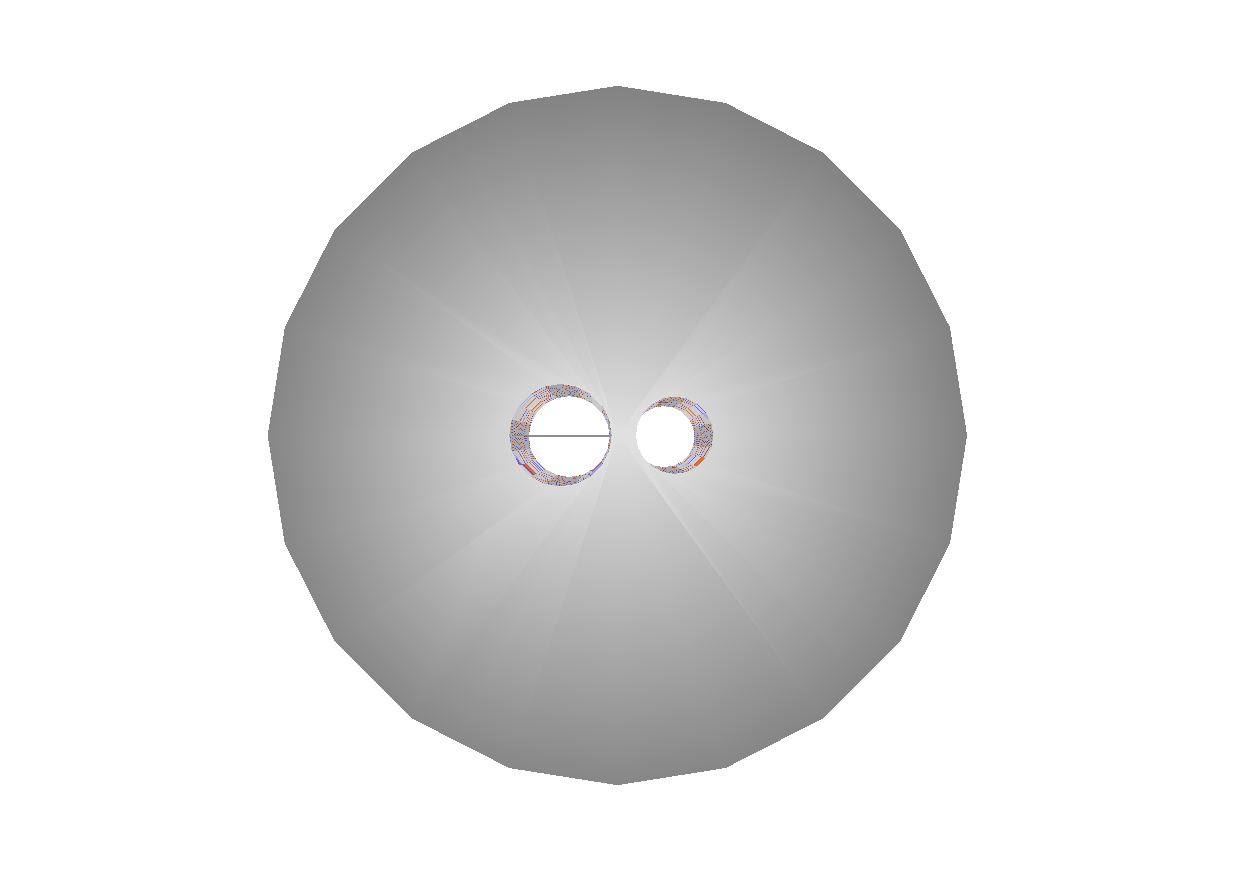
\includegraphics[width=\textwidth]{beamcal_plug}
                        \caption{Full plug region}
                        \label{fig:beamcal_plug}
                    \end{minipage}
                    \begin{minipage}{0.3\textwidth}
                        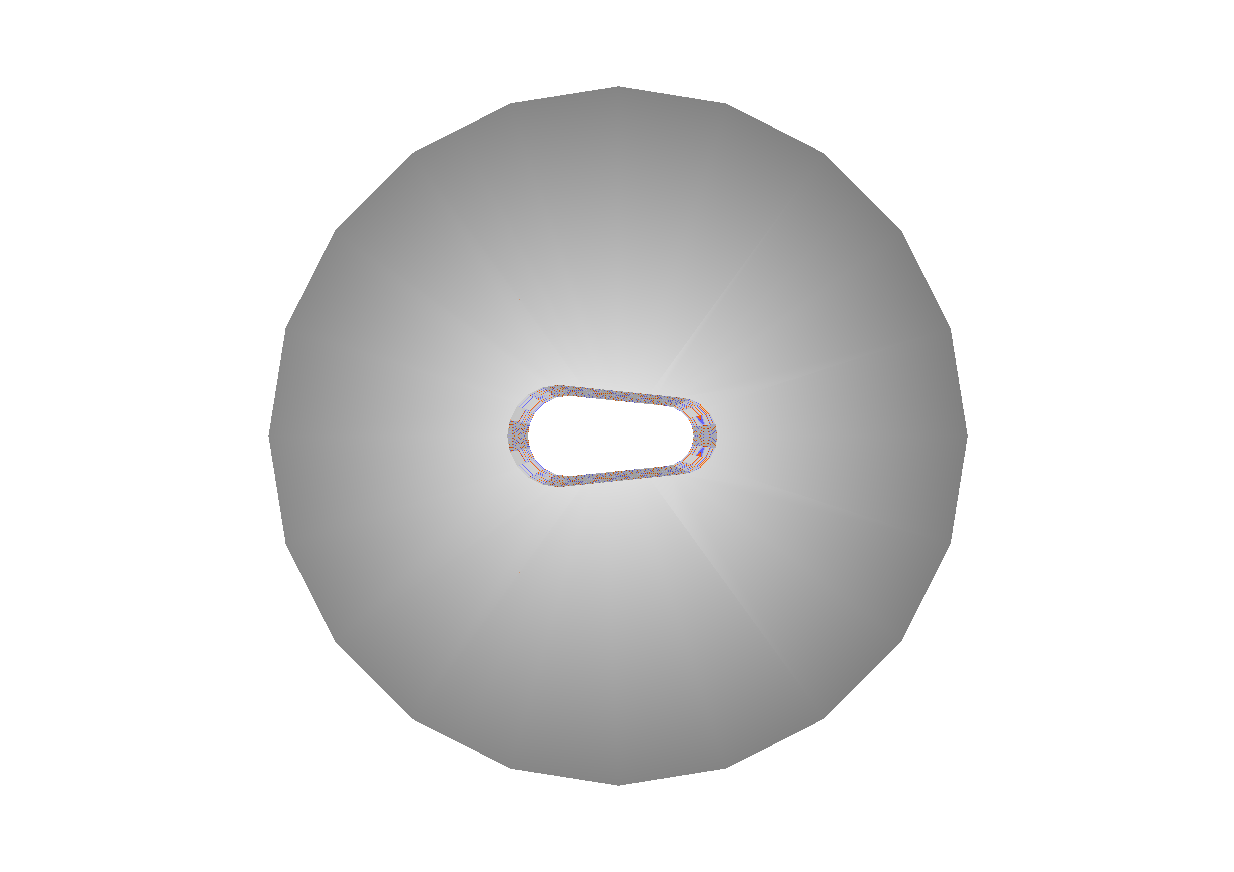
\includegraphics[width=\textwidth]{beamcal_wedge}
                        \caption{Wedge cutout}
                        \label{fig:beamcal_wedge}
                    \end{minipage}
                    \begin{minipage}{0.3\textwidth}
                        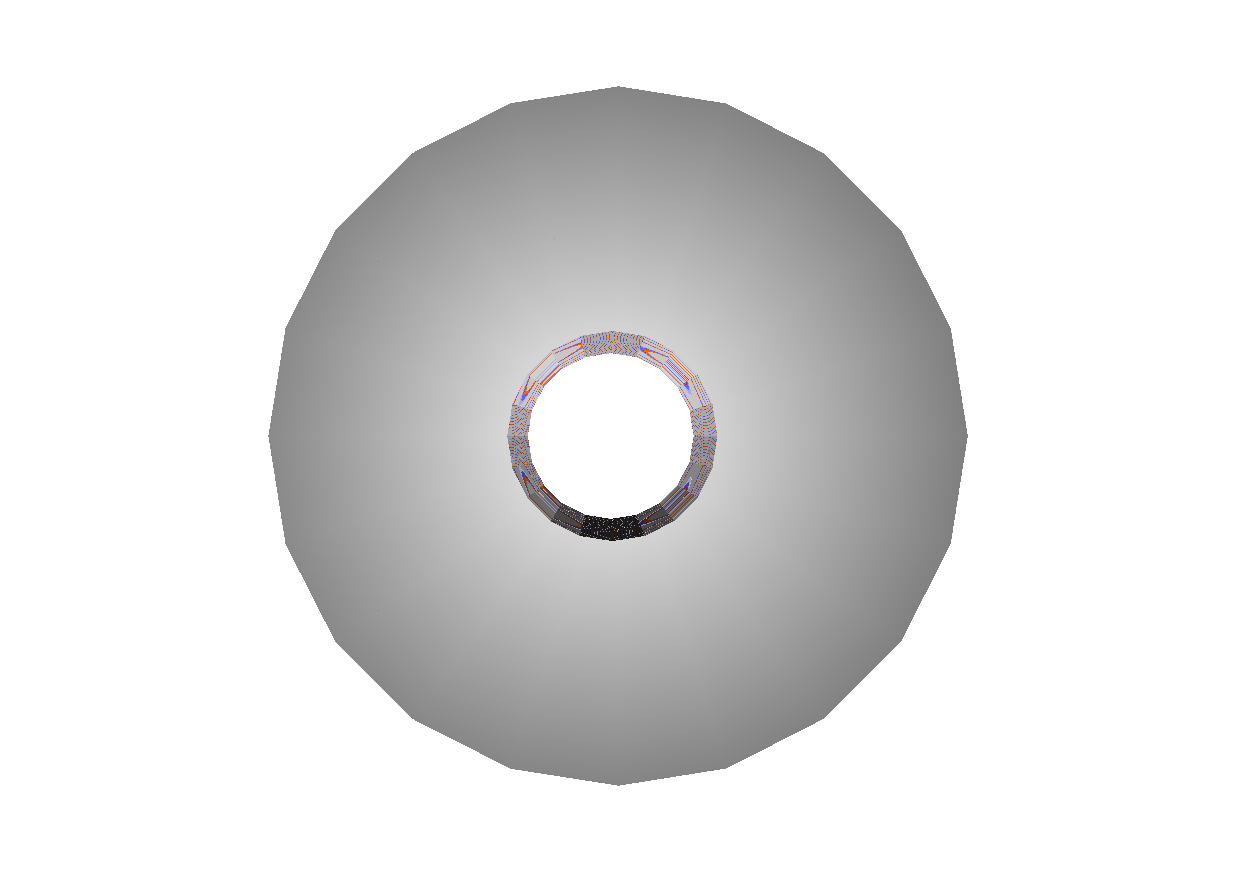
\includegraphics[width=\textwidth]{beamcal_circle}
                        \caption{Circle cutout}
                        \label{fig:beamcal_circle}
                    \end{minipage}
                \end{figure}

                \begin{figure}[h]
                    \centering
                    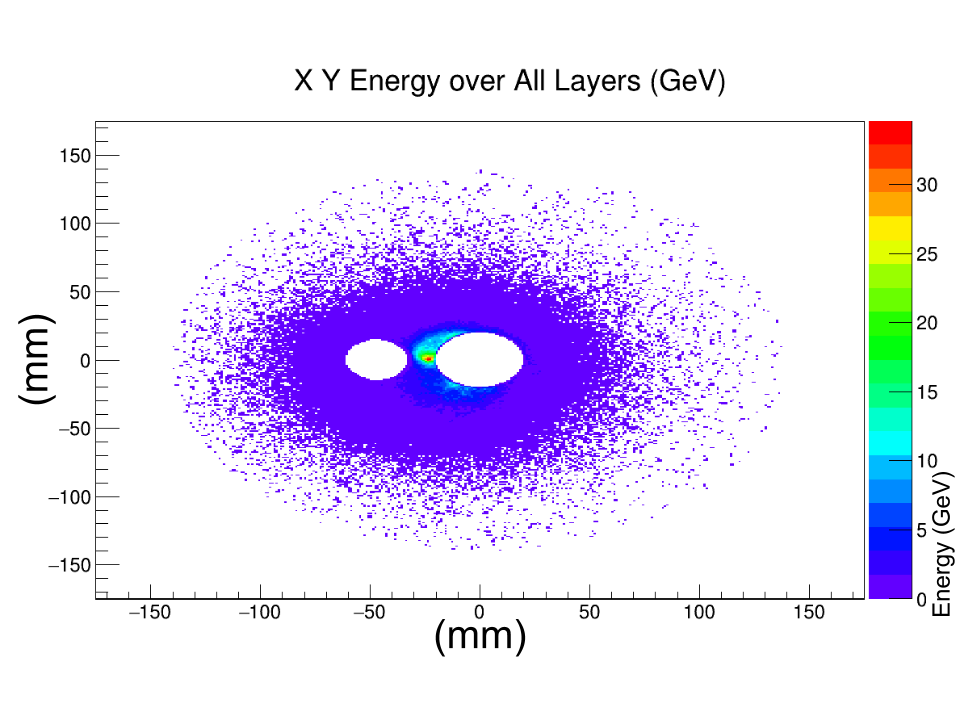
\includegraphics[width=\textwidth]{beamcal_energy_xy}
                    \caption{Energy Deposited on BeamCal from Pairbackground event}
                    \label{fig:beamcal_energy_xy}
                \end{figure}

                As discussed previously, the BeamCal is hit with a very large amount of energy. The overwhelming majority of the energy is deposited in the central area of the BeamCal, between the two beam pipes, as apparent in figure \ref{fig:beamcal_energy_xy}. This central location is referred to as the plug region. Removing all or part of the plug region thus has the potential to reduce the energy incident on the face of the BeamCal, and consequently reduce the albedo effect into the Vertex Detector. There are three proposed designs for the plug region (shown in figures \ref{fig:beamcal_plug}, \ref{fig:beamcal_wedge}, and \ref{fig:beamcal_circle}) which remove progressively more detector material. In theory, these designs should provide lower occupancy in the vertex detector, but the cost to the BeamCal is not yet known.


            %in: albedo, vertex, beamcal
            %out: what is anti-did, why we want it/don't want it, Tom's study
            \subsection{Anti-Did Magnetic Field}
                In response to the problem of albedo from the BeamCal into the Vertex Detector, an engineering team proposed the use of a magnetic field known as the DiD, as well as its counterpart, the anti-DiD. The idea of the anti-Did is to redirect low-energy background particles such that they are funneled into the outgoing beampipe of the BeamCal. By redirecting these particles, the particles hitting the BeamCal are reduced, which reduces the albedo into the Vertex Detector. However, the anti-DiD field is very expensive, and has the potential to cause a number of problems with physics analysis. Additionally, a study performed by Thomas Markiewicz \cite{anti-did} suggested that the anti-DiD field could actually be increasing energy deposition outside of the plug region, only causing improvement in a limited area of the detector. For these reasons, a detailed study of the effects of the anti-DiD field on the BeamCal and Vertex Detector is necessary.


        \section{Goals of the Study} %TODO: move this to abstract
            The objective of this study will be to update the Interaction Region of the SiD to the most modern and up-to-date specifications, directly using the designs of the SiD's top engineer \cite{excel}. Following from this, the three aforementioned changes will be implemented one at a time, analyzing the effects on the performance of the Vertex Detector and Beam Calorimeter. 





    \chapter{Creating New SiD Models}
        \section{Updating the Old SiD Model}
            
            %in: what is sid, what are we doing (geom changes, vertex/beamcal study)
            %out: need to update sidloi3
            The ultimate goal of this study was to analyze new modification to the SiD model. However, before we could look into the future of the SiD, we had to take it out of the past. Prior to my modifications, the most up-to-date simulation model of the SiD was the SiDloi3 model. However, the SiDloi3 model was written in 2011, and numerous changes to the SiD's engineering design had been made since, rendering SiDloi3 outdated. Thus, the first order of business was to ensure that the simulation model was matched to the current engineering design; at least, the aspects of it we were concerned with. As discussed in the introduction, this study focused exclusively on the interaction region of the detector, and as such only the interaction region was fully updated. But even with the scope of the project restricted, the update was no simple task.

            \begin{figure}[h] 
                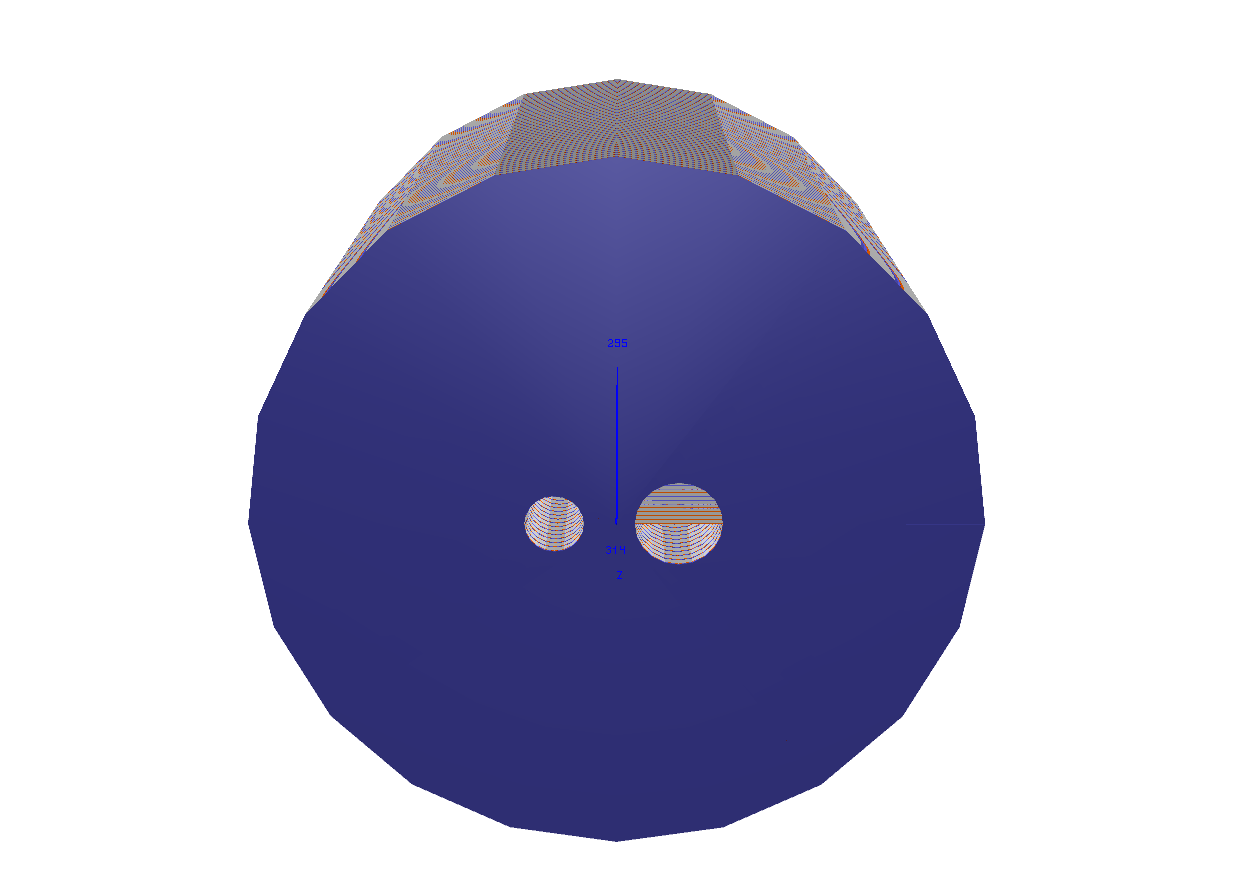
\includegraphics[width=0.7\textwidth]{beamcal_zaxis}
                \centering
                \caption{BeamCalorimeter concentric about z-axis}
                \label{fig:beamcal_zaxis}
            \end{figure}
            \begin{figure}[H] 
                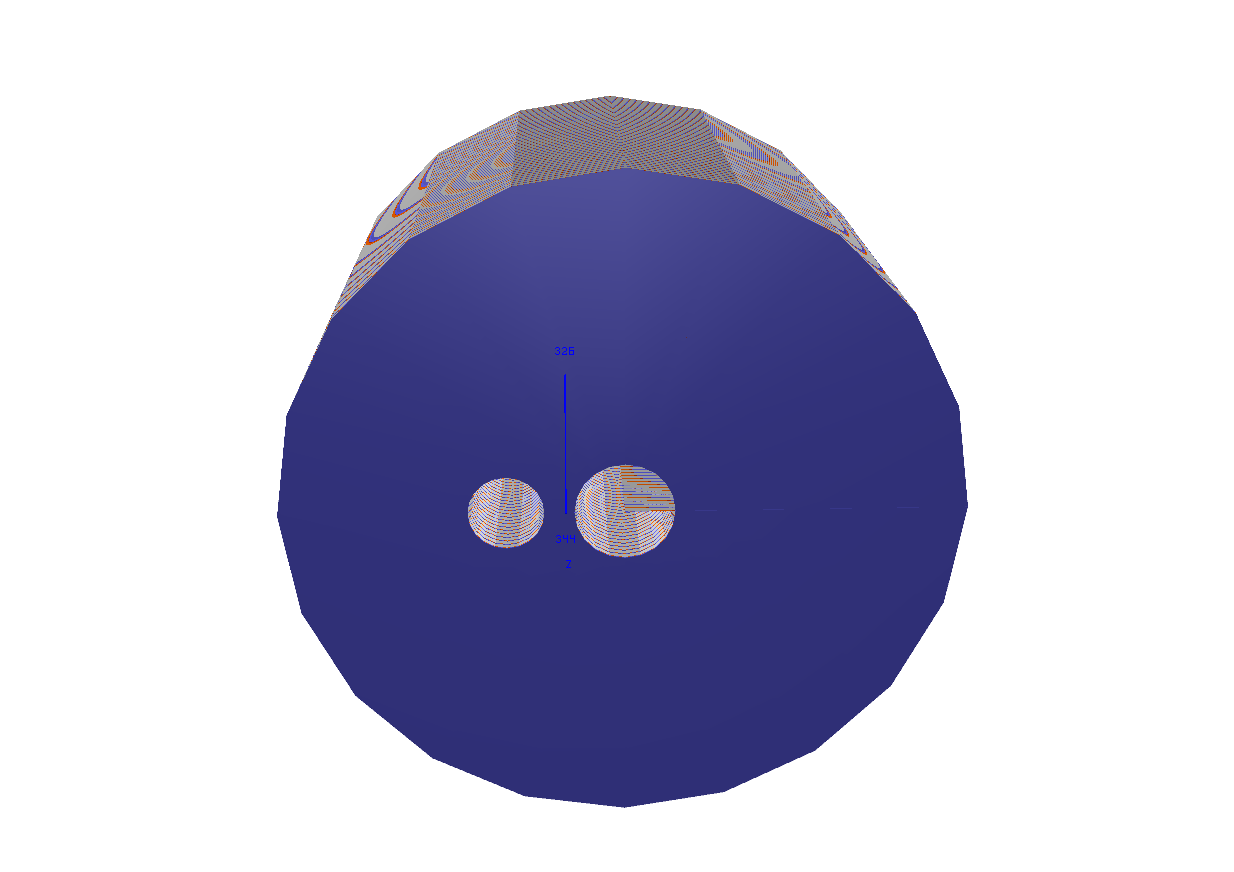
\includegraphics[width=0.7\textwidth]{beamcal_aligned}
                \centering
                \caption{BeamCalorimeter concentric about outgoing beampipe.}
                \label{fig:beamcal_aligned}
            \end{figure}
            \begin{figure}[H] 
                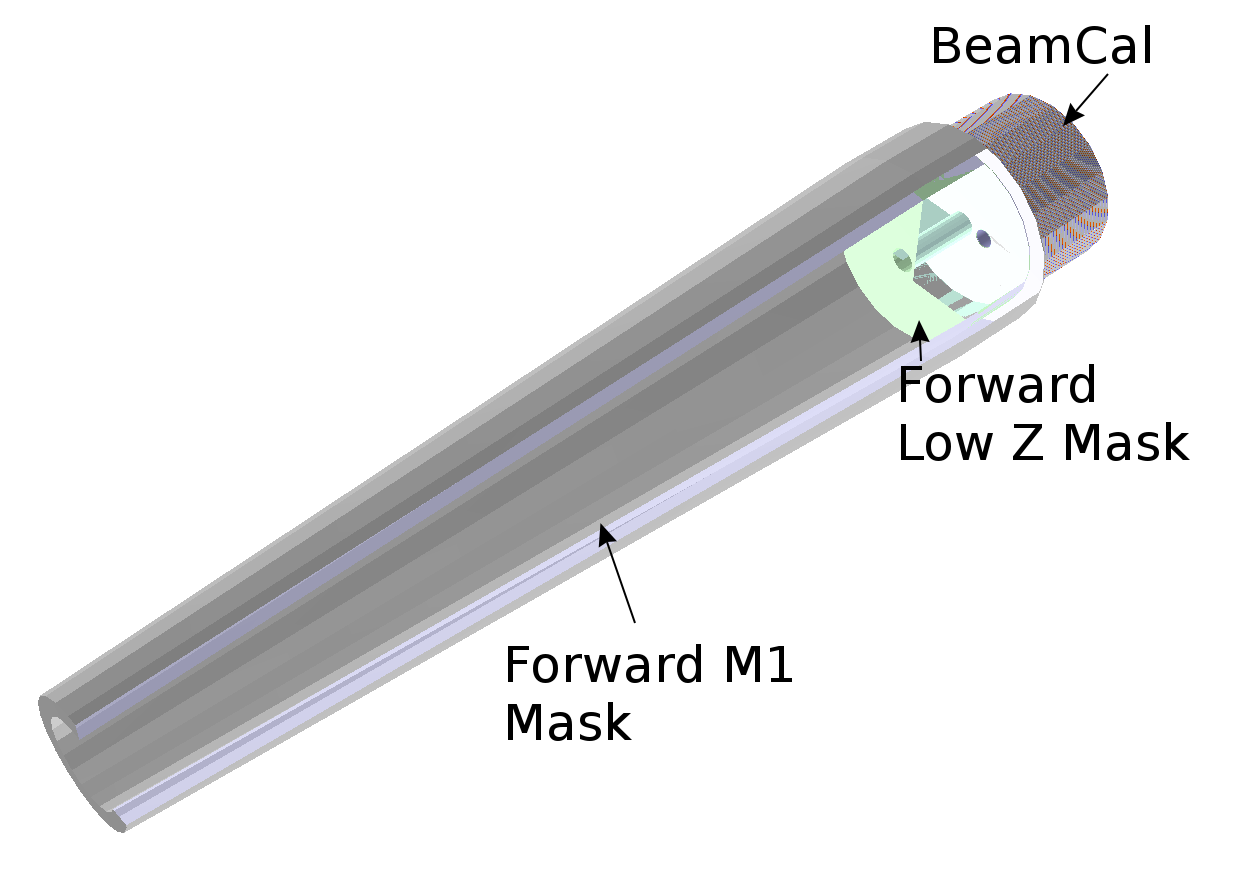
\includegraphics[width=0.7\textwidth]{beamcal_masks}
                \centering
                \caption{BeamCalorimeter with associated masks}
                \label{fig:beamcal_masks}
            \end{figure}

            %in: beamcal
            %out: beamcal alignment, geometry creation process, necessity of code altering
            The most pressing change by far was the realignment of the BeamCal. In the SiDloi3 model, the BeamCal was designed to be concentric about the simulation space's z-axis (figure \ref{fig:beamcal_zaxis}). The most recent engineering designs however (provided by Thomas Markievicz), place the BeamCal concentric about the outgoing beampipe (figure \ref{fig:beamcal_aligned}). In general, modifications to the SiD model are made by editing a specific xml file titled "compact.xml". The modified compact is then run through a program called GeomConverter, which is an extension of the Java based LCSim (Linear Collider Simulator) framework. However, the GeomConverter package did not support off-center alignments of any detector elements, requiring significant modifications be made to the source code (the full source code changelog can be found in section \ref{sect:geom_changes}). Once the changes were made, and the BeamCal appropriately realigned to be concentric about the outgoing beampipe, it was a simple matter to similarly realign the BeamCal's associated masks: the ForwardLowZ mask, and the ForwardM1 mask, both visible in figure \ref{fig:beamcal_masks}). 

            \begin{figure}[h] 
                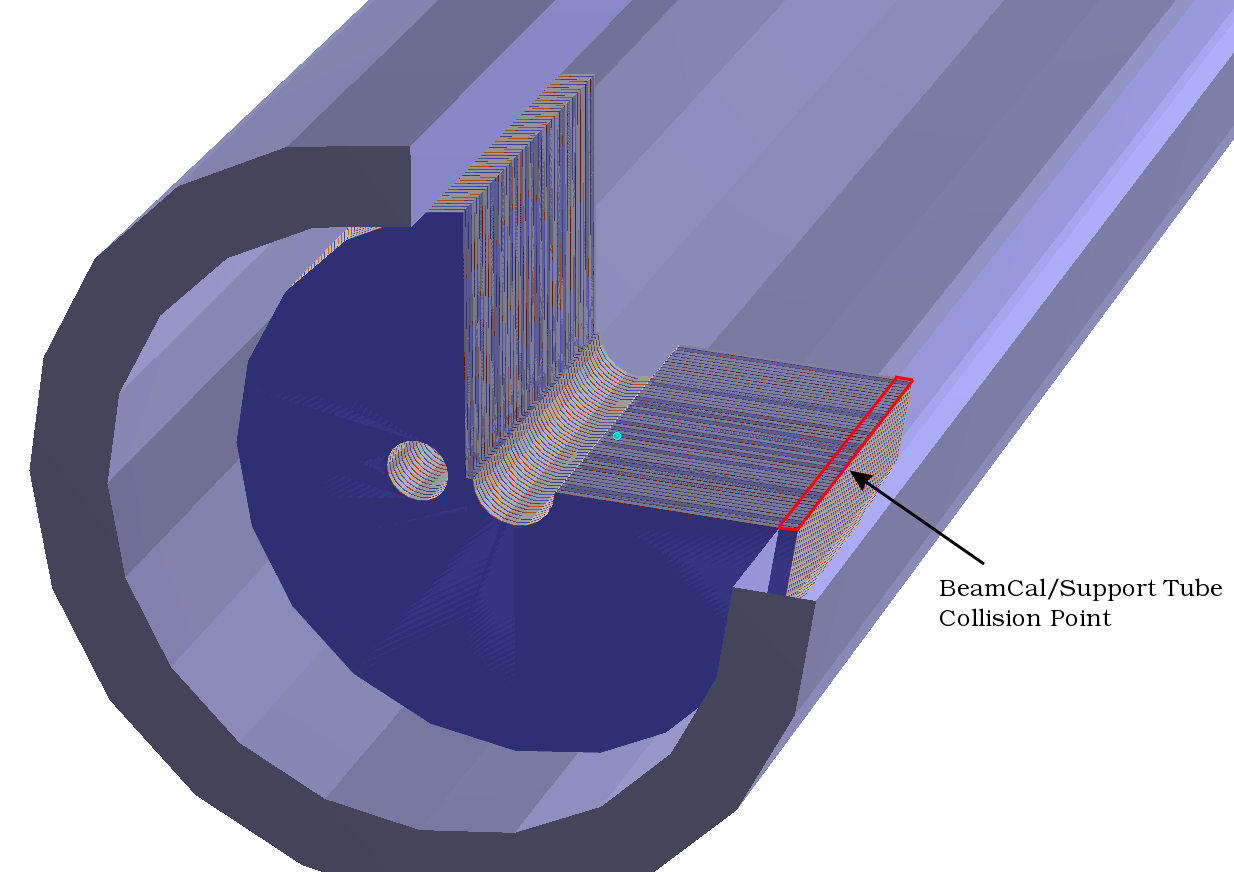
\includegraphics[width=0.7\textwidth]{beamcal_collide}
                \centering
                \caption{BeamCalorimeter Colliding with Forward Support Tube}
                \label{fig:beamcal_collide}
            \end{figure}

            %in: beamcal, need for code altering, Tom's engineering designs, brief knowledge of ecal, hcal, and muon detector
            %out: I had to change extra stuff in xml
            Hypothetically speaking, once the BeamCal and its masks were properly realigned, the study could have proceeded forward without any further updates to the SiD model. Unfortunately, usage of CERN ROOT's gdml viewer revealed that the realignment of the BeamCal caused it to collide with a support tube structure (figure \ref{fig:beamcal_collide}). It was quickly apparent that altering the support tube structure alone would be useless, as this would result in even more collisions with a myriad of other SiD components. Thus, additional modifications to the detector elements surounding the support tube (notably the Ecal, Hcal, and Muon Detector) were needed. While these modifications were in line with Markievicz's engineering designs, they only constitute partial modifications to the non-interaction region elements. Most of the non-interaction region elements are still using outdated designs.

            %in: beamcal, need for code altering, lumical, sitracker.
            %out: I had to change even more extra stuff in detector
            In addition to the BeamCal, it was also decided that the LumiCal should be updated. The reason for this is that the LumiCal places constraints on the angles at which particles can hit the BeamCal. Updating the LumiCal brought about a problem of its own though. In the most recent engineering designs, the LumiCal was moved closer to the interaction point, such that the outermost layer of the SiTracker Endcap surrounded it. While this poses no realistic problem, the GEANT4 simulation software would not tolerate it, as this placed the LumiCal within a virtual boundry called the "Tracking Volume", which surrounds the SiTracker. In short, the Tracking Volume causes all elements inside it to store significantly more simulation information. Because the LumiCal is a calorimeter, and therefore induces a large shower of particles, storing the additional information from the Tracking Volume caused excessive RAM usage, making simulations impossible. As a result, we were forced to move the outermost layer of the SiTracker endcap (allowing us to shrink the Tracking Volume) closer to the interaction point, so that it no longer surrounded the LumiCal. Upon finishing this adjustment though, the SiD forward region was fully up to date, and new design decisions could be implemented (the full geometry changelog can be found in section \ref{sect:compact_changes}).


        \section{Experimenting with New SiD Models}

            %in: sidloi3, why we're making changes, what the L*, plug region, and anti-did are, set of geometry lcdds used, what GEANT4 is, what SLAC is, what and lsf computing cluster is. what a pairbackground event is, what the luminosity upgrade is, what a train is
            %out: what a signal event is, how slcios were generated for the beamcal and vertex.
            \subsection{Simulation: From stdhep to slcio}
                With the sidloi3 sufficiently updated, experiments on the various alternate configurations could begin. The three geometric changes, as discussed in section \ref{sect:sid_mods}, are the length of the L*, the configuration of the plug region of the BeamCal, and the inclusion of an anti-did field. Five lcdd simulation geometries were generated (using the same tools discussed in the previous section) in order to analyze these changes. The 'control' case was using the new 4.1 meter L* with the full plug region and no anti-DiD field. The other four were variations on this. One used the 3.5 meter L*, one used the anti-DiD field, and the remaining two used the alternate plug regions. For the two detector elements studied (BeamCal and Vertex Detector), two simulation methods were used. 

                For the BeamCal, these lcdd files were run through SLIC (a GEANT4 wrapper), on SLAC's LSF computing cluster, in order to generate 300 pairbackground events and 10,000 ad-hoc high energy signal events per geometric configuration. The discrepency in event numbers is due to the high time demands of generating pairbackgrounds, coupled with the fact that pairbackgrounds are not the main focus of the BeamCal study (thus requiring less rigorous statistics). It is worth mentioning here just what these 'ad-hoc' electrons are. They are high energy electrons that are generated at the IP with extremely low transverse momentum. They are \textit{not} real, physical events. They are merely a useful tool for first order studies of a detector's tagging efficiency.

                The simulations performed for the Vertex detector underwent a different process. The studies for the Vertex Detector are solely dependant on pairbackground events, and demand the rigorous statistics the BeamCal was able to avoid. As already mentioned, pairbackgrounds are very computationaly intensive and time consuming to generate, to a degree the SLAC cluster is unequipped for. As such, I turned to PNNL physicist and SiD tech support Jan Strube. Jan then used the Open Science Grid (OSG) to generate 2500 pairbackground events per geometric configuration (2500 being the rough number of bunch crossings in a train, post luminosity upgrade). Additionally, in order to save hard disk space, Jan stripped the pairbackground simulation files of all information except that pertaining to the Vertex Detector. 

            %in: what slcio files are, what pixellation is
            %out: how the vertex occupancy was analyzed (brief), how beamcal tagging works
            \subsection{Analyzing the Simulations}
                The end result of both simulation methods was a large collection of slcio files, which contained the details of the various simulations. From here, the LCSim framework was used as a backend to a personal suite of analysis code I wrote to study the physics of the BeamCal and Vertex Detector. For the Vertex Detector, a program was used to pixellate the hits on the detector and then perform fractional occupancy analysis on the resulting pixels as function of various parameters (discussed further in the Analysis section). For the BeamCal, the analysis is more complicated.
                
                The analysis of the BeamCal studies the efficiency of its signal reconstruction efficiency. It is appropriate then to provide an overview of how the reconstruction algorithm works (a more thorough discussion can be found in \cite{bogert_thesis}). The algorithm first populates the pixels of the BeamCalorimeter with the information provided by both the signal electron and the pairbackground lcdd files, one event at a time. It then performs a sweep across the tenth layer of the BeamCal, aggregating the pixels into clusters called 'pallets'. It selects the pallets with the top 50 highest background-subtracted energies deposited in them. The selected pallets are then 'extended' to include all pixels in the same x/y locations in layers 10 through 40, summing the raw energy of all included pixels to produce a new structure refered to as a 'cylinder'. The 50 cylinders are iterated through. If the background-subtracted energy of any of the cylinders exceeds a particular standard deviation (sigma cut), then the event is deemed to contain a signal event and rejected. The sigma cut is chosen such that no more than ten percent of all events which do \textit{not} contain a signal event are rejected. This algorithm's efficiency in correctly identifying signal electrons, particularly as a function of radius, was then studied and compared across the range of architectural configurations, using three different measures of efficiency.

                By measures of efficiency, I mean instrumental efficiency, geometric efficiency, and total efficiency. Instrumental efficiency is the frequency with which the tagging algorithm correctly identifies events where the high energy electron/positron \textit{hits the BeamCal}. If the electron/positron misses the BeamCal entirely then the algorithm is unable to tag it. In instrumental efficiency though, only events where the electron/positron hit the BeamCal count towards the efficiency rating. Conversly, geometric efficiency ignores the tagging algorithm entirely, determining only whether or not an electron/positron hit the BeamCal. The combination of these two, the frequency of how often the algorithm correctly tags \textit{any} electron/positron (including those which miss the BeamCal), is reffered to as the total efficiency. In the following analysis, the total efficiency of the architectures is studied, and then disected by separetly comparing the instrumental and geometric efficiencies.





    \chapter{Analysis}
        \section{L star}
            \subsection{Beam Calorimeter}
                \begin{figure}[H] 
                    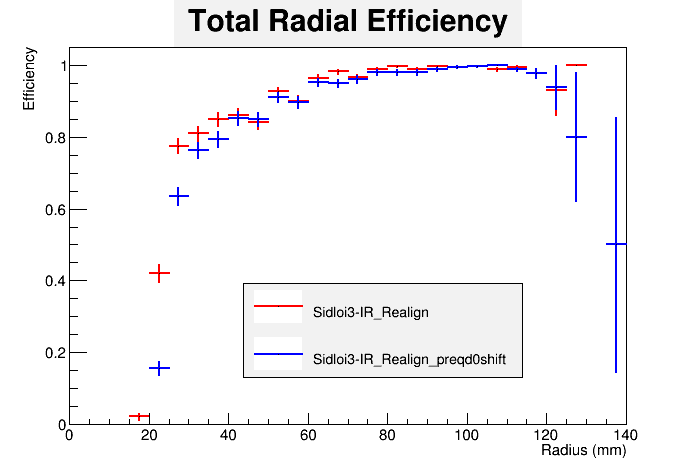
\includegraphics[width=\textwidth]{RadialEfficiencyFP_total}
                    \centering
                    \caption{}
                    \label{fig:lstar_beamcal_total}
                \end{figure}
                \begin{figure}[H]
                    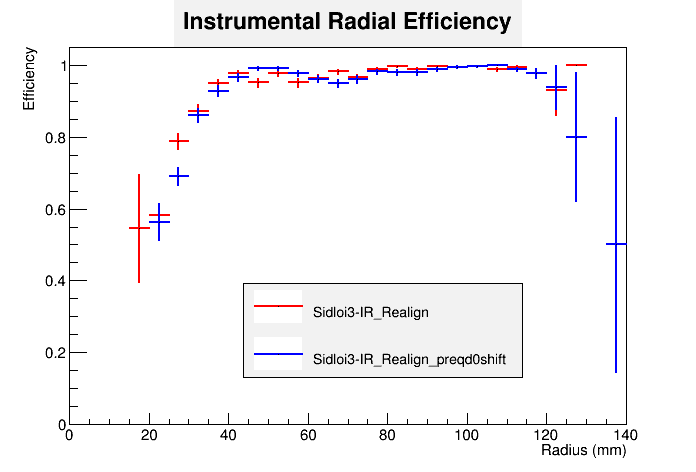
\includegraphics[width=\textwidth]{RadialEfficiencyFP_instrumental}
                    \centering
                    \caption{}
                    \label{fig:lstar_beamcal_inst}
                \end{figure}
                \begin{figure}[H]
                    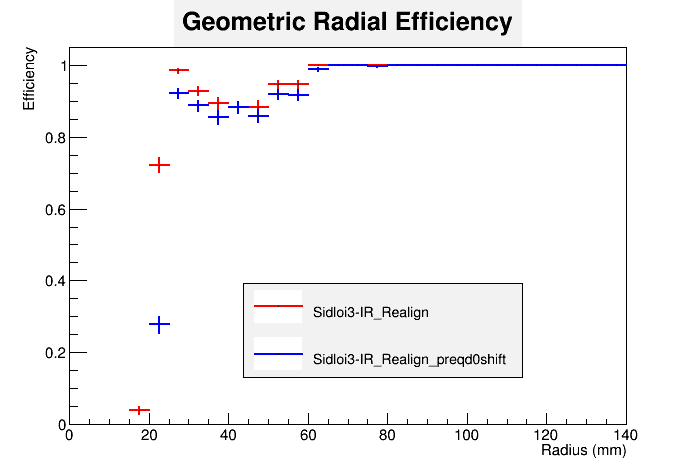
\includegraphics[width=\textwidth]{RadialEfficiencyFP_geometric}
                    \centering
                    \caption{}
                    \label{fig:lstar_beamcal_geom}
                \end{figure}

                As visible in figure \ref{fig:lstar_beamcal_total}, moving the BeamCal further away from the IP only has a marginal effect, except at the innermost radii. Looking at figures \ref{fig:lstar_beamcal_inst} and \ref{fig:lstar_beamcal_geom}, it is apparent that this is a geometric effect. At a further distance from the IP, the inner radii of the BeamCal corresponds to a lower angle in theta. This means that a number of very low angle electrons are hitting the BeamCal at the 4.1 meter L* position, which missed the BeamCal at the 3.5 meter L*, resulting in more electrons being detected.
                
            \subsection{Vertex Detector} 
                \begin{figure}[H]
                    \centering
                    \begin{minipage}{0.4\textwidth}
                        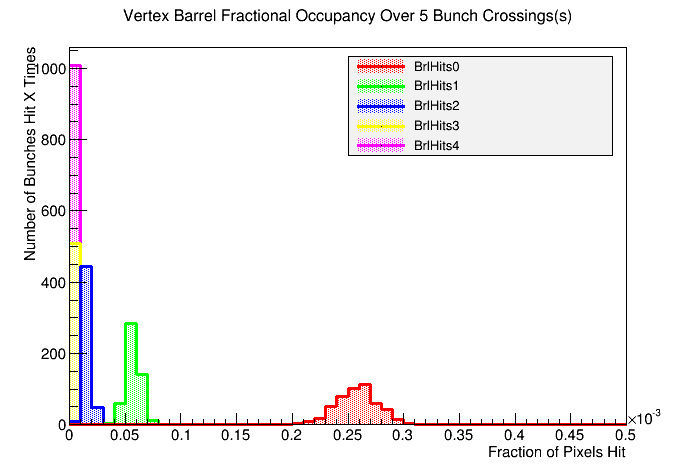
\includegraphics[width=\textwidth]{Voccupancy_sidloi3_IR_realign_preqd0shift_5B_ps30_1510212229_brl}
                        \caption{Vertex Barrel 3.5 meter L*}
                        \label{fig:lstar_vertex_brl_3.5}
                    \end{minipage}
                    \begin{minipage}{0.4\textwidth}
                        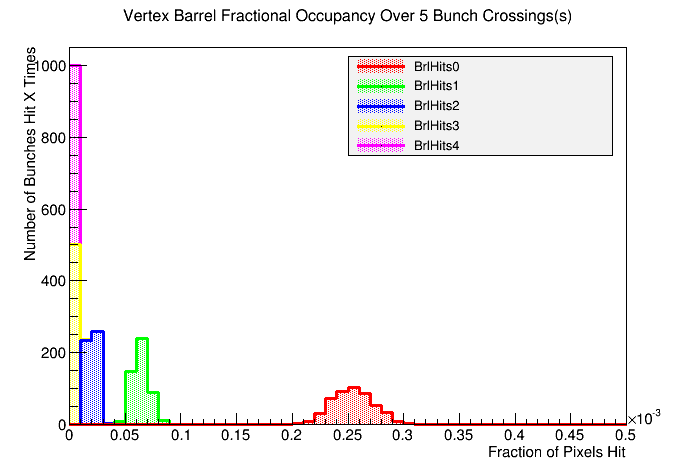
\includegraphics[width=\textwidth]{Voccupancy_sidloi3_IR_realign_5B_ps30_1510211229_brl}
                        \caption{Vertex Barrel 4.1 meter L*}
                        \label{fig:lstar_vertex_brl_4.1}
                    \end{minipage}
                \end{figure}
                \begin{figure}[H]
                    \centering
                    \begin{minipage}{0.4\textwidth}
                        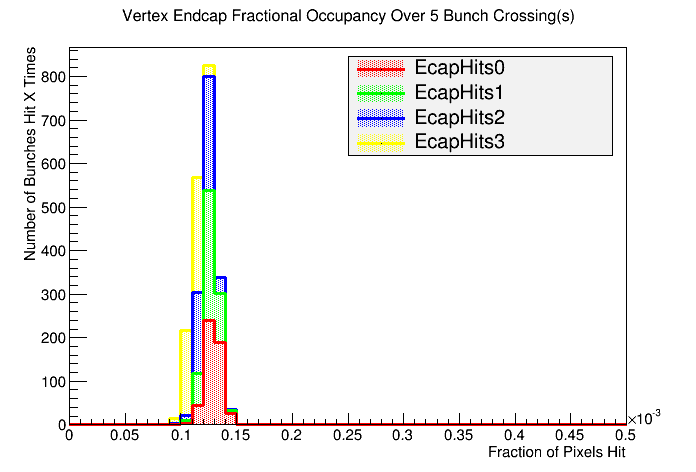
\includegraphics[width=\textwidth]{Voccupancy_sidloi3_IR_realign_preqd0shift_5B_ps30_1510212229_ecp}
                        \caption{Vertex Endcap 3.5 meter L*}
                        \label{fig:lstar_vertex_ecp_3.5}
                    \end{minipage}
                    \begin{minipage}{0.4\textwidth}
                        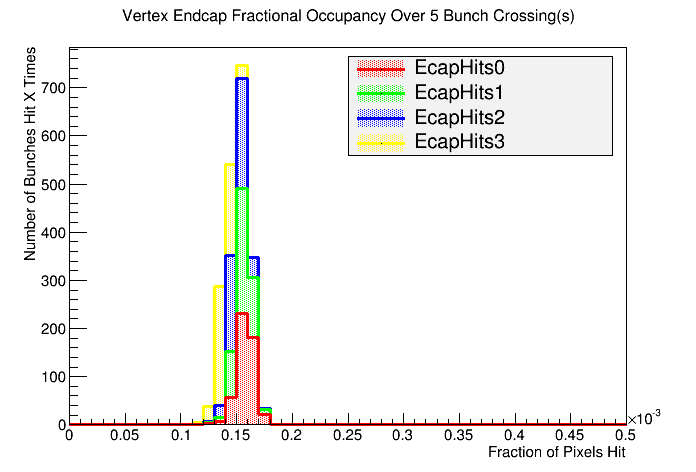
\includegraphics[width=\textwidth]{Voccupancy_sidloi3_IR_realign_5B_ps30_1510211229_ecp}
                        \caption{Vertex Endcap 4.1 meter L*}
                        \label{fig:lstar_vertex_ecp_4.1}
                    \end{minipage}
                \end{figure}
                The effect of the BeamCal movement on the Vertex Detector Occupancy is virtually non-existant. Figures \ref{fig:lstar_vertex_brl_3.5} and \ref{fig:lstar_vertex_brl_4.1} show that the Vertex Barrel has no noticeable change. Figures \ref{fig:lstar_vertex_ecp_3.5} and \ref{fig:lstar_vertex_ecp_4.1} show that there is a very slight change to the endcap, noteably that the 4.1 meter L* has slightly higher occupancy than the 3.5 meter L*. The reason for the change is likely the same as that which increased tagging efficiency in the BeamCal. That is, the BeamCal has slightly better angular coverage for low theta particles. This would result in more background particles hitting the BeamCal at low radii, causing slightly higher albedo levels.

            \subsection{Conclusion}
                As stated previously, the decision to move the L* from 3.5 to 4.1 meters has already been finalized, so these studies are unable to influence it. Luckily however, it seems that the change only improved matters. The BeamCal now operates more efficiently at low radii, and the Vertex Detector, while not performing any better, does not really perform any worse either.


        \section{Plug Region}
            \subsection{Beam Calorimeter}
                \begin{figure}[H] 
                    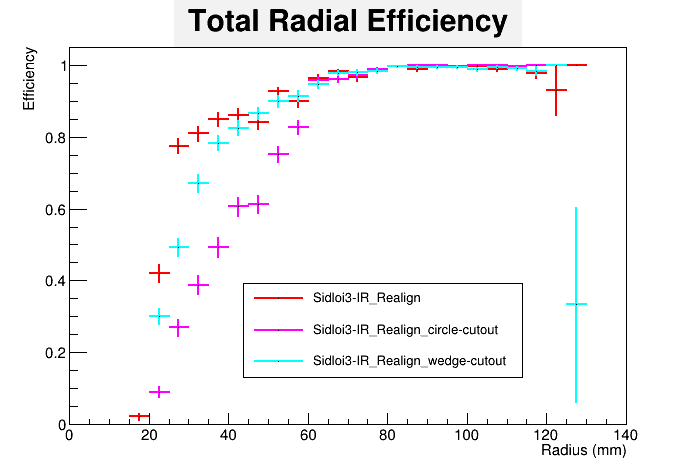
\includegraphics[width=\textwidth]{RadialEfficiency_total_geom}
                    \centering
                    \caption{}
                    \label{fig:geom_beamcal_total}
                \end{figure}
                \begin{figure}[H]
                    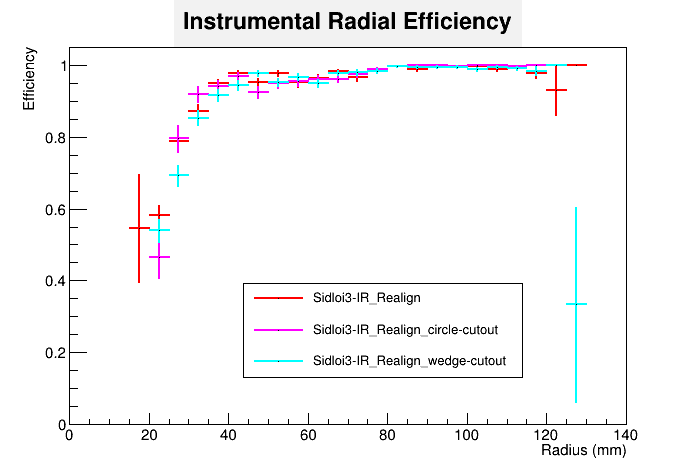
\includegraphics[width=\textwidth]{RadialEfficiency_instrumental_geom}
                    \centering
                    \caption{}
                    \label{fig:geom_beamcal_inst}
                \end{figure}
                \begin{figure}[H]
                    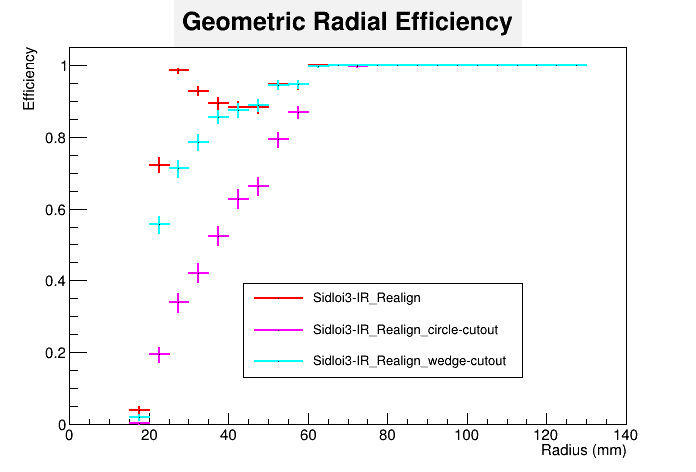
\includegraphics[width=\textwidth]{RadialEfficiency_geometric_geom}
                    \centering
                    \caption{}
                    \label{fig:geom_beamcal_geom}
                \end{figure}

                As expected, removing part of the BeamCal causes massive drops in performance near the removed region, as visible in figure \ref{fig:geom_beamcal_total}. Additionally, the performance drop increases with the more liberal circular cutout. Outside of the inner radii, the performance is unchanged, as was also expected. The effect on the BeamCal is entirely geometric(\ref{fig:geom_beamcal_geom}), with no significant effects on the instrumental efficiency (\ref{fig:geom_beamcal_inst}).
                
            \subsection{Vertex Detector} 
                \begin{figure}[H] 
                    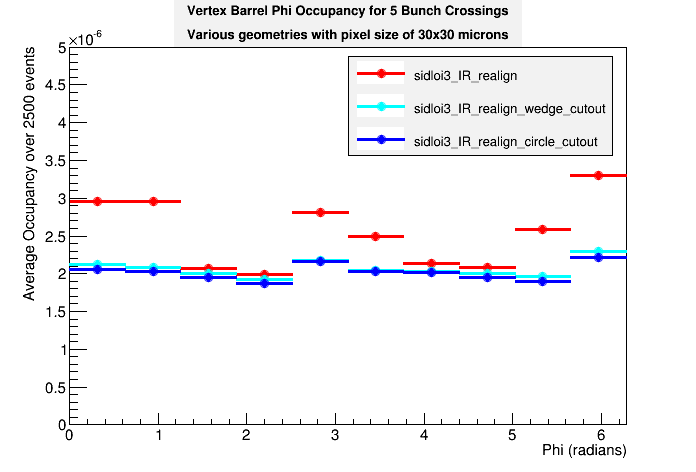
\includegraphics[width=\textwidth]{VradOccupancy_plug_brl}
                    \centering
                    \caption{Vertex Barrel Plug Region}
                    \label{fig:plug_vertex_brl}
                \end{figure}
                \begin{figure}[H] 
                    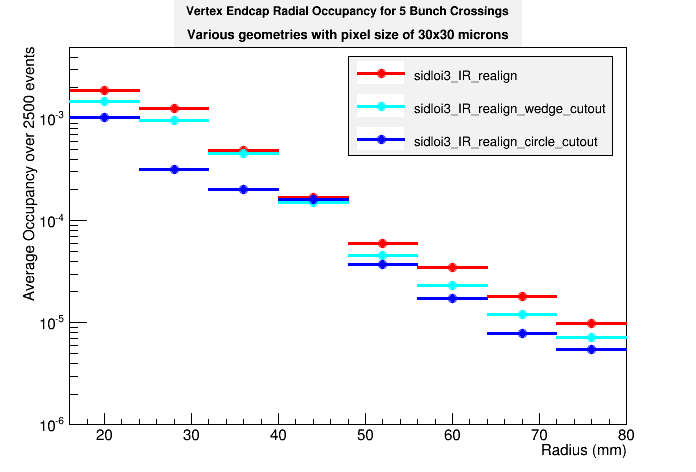
\includegraphics[width=\textwidth]{VradOccupancy_plug_ecp}
                    \centering
                    \caption{Vertex Endcap Plug Region}
                    \label{fig:plug_vertex_ecp}
                \end{figure}
                The backscatter effect from the BeamCal into the Vertex Detector is dependent on there being something for the particles to scatter backwards off of. It makes perfect sense then, that removing material from the BeamCal would decrease the occupancy in the Vertex Detector, visible in figures \ref{fig:plug_vertex_brl} and \ref{fig:plug_vertex_ecp}, with the circle cutout resulting in even lower occupancy levels.
                

            \subsection{Conclusion} 
                 It would certainly prove beneficial to the Vertex Detector's performance if part of the plug region could be removed, but whether or not the losses to the BeamCal are tolerable is still an open question. The events used to analyze them in this study are, as mentioned previously, not real physical events. The event type that this algorithm really needs to be used for is the gamma-gamma to hadron event type. At the time of writing this, studies on the gamma-gamma to hadron events have begun, but are many months from completion. A more thorough decision on the plug region will be made once the plug region's effect on gamma-gamma to hadron tagging is studied.

        
        \section{Anti-DiD}
            \subsection{Beam Calorimeter}
                \begin{figure}[H] 
                    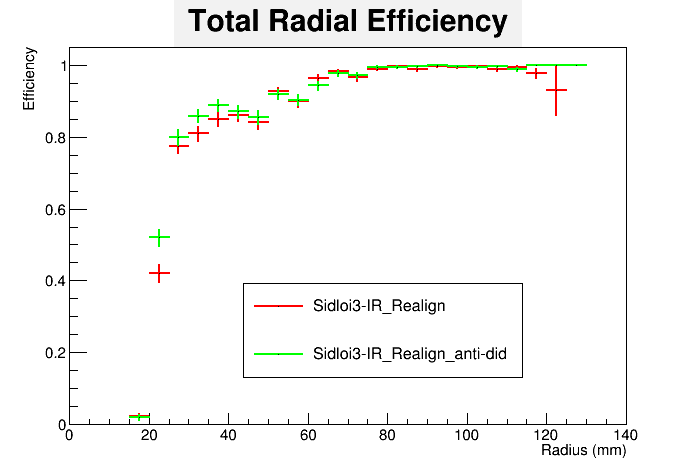
\includegraphics[width=\textwidth]{RadialEfficiency_total_did}
                    \centering
                    \caption{}
                    \label{fig:did_beamcal_total}
                \end{figure}
                \begin{figure}[H]
                    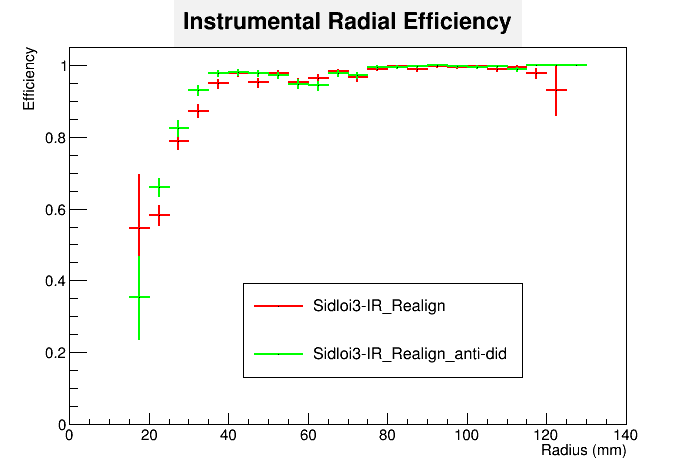
\includegraphics[width=\textwidth]{RadialEfficiency_instrumental_did}
                    \centering
                    \caption{}
                    \label{fig:did_beamcal_inst}
                \end{figure}
                \begin{figure}[H]
                    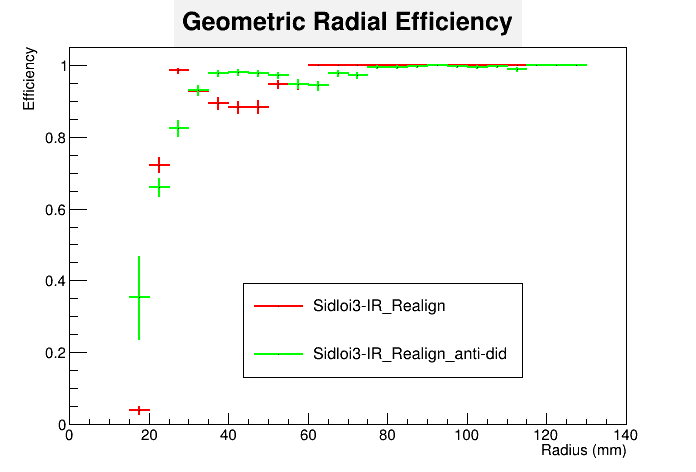
\includegraphics[width=\textwidth]{RadialEfficiency_geometric_did}
                    \centering
                    \caption{}
                    \label{fig:did_beamcal_geom}
                \end{figure}

                As visible in figure \ref{fig:did_beamcal_total}, the anti-DiD field improves the BeamCal's efficiency by a noticeable margin at all radii. The reason for this is likely that the anti-DiD field is funneling a substantial portion of the background energy into the outgoing beampipe. Without this background energy hitting the BeamCal, the tagging algorithm is able to more easily identify signal events.

            \subsection{Vertex Detector}
                \begin{figure}[H] 
                    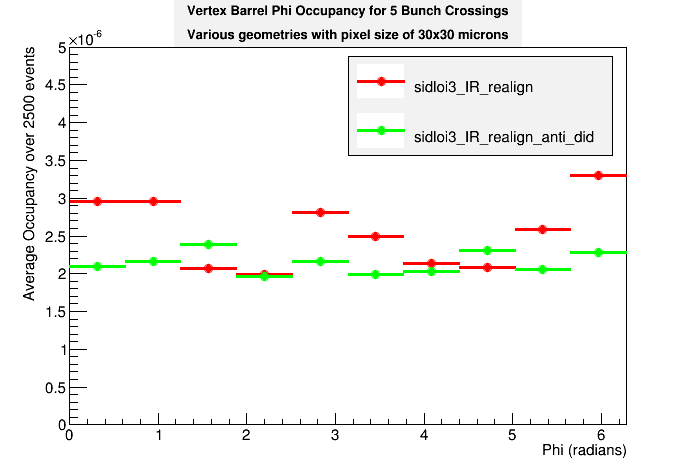
\includegraphics[width=\textwidth]{VradOccupancy_base_brl}
                    \centering
                    \caption{Vertex Barrel Plug Region}
                    \label{fig:did_vertex_brl}
                \end{figure}
                \begin{figure}[H] 
                    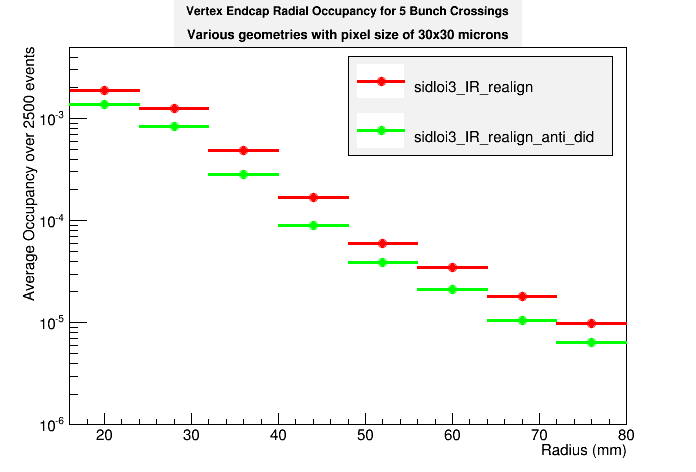
\includegraphics[width=\textwidth]{VradOccupancy_base_ecp}
                    \centering
                    \caption{Vertex Endcap Plug Region}
                    \label{fig:did_vertex_ecp}
                \end{figure}
                Figures \ref{fig:did_vertex_brl} and \ref{fig:did_vertex_ecp} shows that the anti-DiD field reduces the occupancy levels in both the barrel and endcap of the Vertex Detector. Just as with the BeamCal tagging efficiency, this improvement results from background particles being sent down the outgoing beampipe. Because a large number of particles now miss the BeamCal, the albedo is reduced, improving occupancy.

            \subsection{Conclusion}
                The anti-DiD field certainly accomplishes its intended goal, by improving performance in both the BeamCal and Vertex Detector. However, the BeamCal and Vertex Detector are not the only considerations for the anti-DiD field. While the anti-Did may be intended for only these two detectors, the field can cause problems with various other parts of the SiD overall. Moreover, the anti-DiD is very expensive, costing on the order of millions of dollars (US). For these reasons, the marginal improvements to the BeamCal and Vertex detector are not worth the costs of installing the anti-DiD field. The conclusion of this study and the SiD collaboration as a whole then is that the anti-Did field will \textbf{not} be included in the final design of the SiD.





    \chapter{Appendices}
        \section{GeomConverter Source Code Changelog} \label{sect:geom_changes}
            \begin{verbatim}
                all files changed are located in:
                lcsim/detector-framework/src/main/java/org/lcsim/geometry/compact/converter/lcdd/


                ForwardDetector.java:
                    This is the file that determines the BeamCal's geometry, as well as the
                    geometry of the polyethylene mask in front of the BeamCal.
                    
                    It was modified in order to allow the BeamCal and its mask to be alligned
                    to the outgoing beampipe.
                    
                    The rotation itself was straightforward, requiring only a few lines of
                    code towards the end to A) rotate the BeamCal by half the crossing angle
                    (0.014 radians, so the BeamCal was rotated by 0.007 radians), and B) 
                    shift the BeamCal in x by [zposition*tan(crossing_angle/2)]. The
                    shift in x was neccessary because the rotation is about the BeamCal's
                    local center, not the global origin. 

                    The catch was the two holes in the BeamCal which needed to be subtracted
                    from the volume for the beampipes. This subtraction is done not just in
                    every layer, but in every slice of material in every layer. The result is
                    effectively the same body of code in three locations to perform the
                    rotated subtraction properly (one for the main beamcal, one for each
                    layer, and one for each slice). 


                util/PhysVol.java:
                    This is the class which is actually interpreted by the program as
                    belonging to the geometry. When a geometric object in the code is generated, the
                    last step is to create a PhysVol object with the geometric object, which
                    is then added to the "mother volume" PhysVol object.

                    This was modified merely to add two convenience functions. There was
                    already a function (setZ) built into it that allowed one to easily set the
                    z-position of a PhysVol object. I simply added two more that did the same
                    thing for x and y. The function for x (setX) was used for the shift
                    mentioned in the ForwardDetector.java, and the setY function was just for
                    completeness.


                PolyconeSupport.java:
                    This is the class which converts, among many other things, the large
                    support tube which encompasses the BeamCal and mask.

                    It was modified to allow it to be alligned to the outgoing beampipe.
                    Oddly, while the BeamCal requires both a rotation and x position be set,
                    the PolyconeSupport only requires rotation, as its axis of rotation
                    appears to be the origin.

                    While the functionality for alignment is still present in the code, later discussion
                    revealed that the support tube should remain alligned to the z-axis, so
                    the functionality is not currently being used.


                CylindricalEndcapCalorimeter.java:
                    This is the class which converts the LumiCal.

                    It was modified to allow alignment to the outgoing beampipe. Like the
                    BeamCal, it requires a rotation and shift-in-x parameter to be aligned
                    correctly. However, the hole in the center of the LumiCal is generated
                    through a different method than the BeamCal holes, which means it does not
                    require any special attention.
            \end{verbatim}


        \section{compact.xml Changelog} \label{sect:compact_changes}
            \begin{verbatim}
                All numbers in units of mm


                Changes made in order to comply with Tom Markiewicz's engineering excel file:

                    EcalBarrel inner radius: 1265 -> 1270
                    EcalEndcap inner radius: 200 -> 216
                    EcalEndcap outer radius: 1294.1 -> 1250

                    HcalBarrel inner radius: 1419 -> 1410
                    HcalBarrel z from origin to edge: 3018 -> 2940

                    HcalEndcap inner radius: 200 -> 216
                    HcalEndcap outer radius: 1458.7 -> 1402
                    HcalEndcap z-min: 1805 -> 1820

                    MuonEndcap zmin: 3028 -> 3030
                    MuonEndcap rmin: 200 -> 211

                    LumiCal zmin: 1680 -> 1557

                    BeamCal outer_r: 129.6 -> 159
                    BeamCal inner_z: 2950 -> 3265
                    BeamCal slice material Tungsten density 24 thickness: 2.71 -> 2.5
                    
                    BeamCal support tube rmin: 155 -> 194
                    BeamCal support tube rmax: 195 -> 211
                    BeamCal support tube zmin: 1820 -> 1700
                    BeamCal support tube zmax: 3235 -> 6773

                    Forward & Backward M1 support:
                        initial: rmin 80 -> 70, rmax 155 -> 100, z 1820 -> 3135
                        final:   rmin 137.8 -> 169, rmax 155 -> 194, z 3135 -> 3125

                    ForwardLowZ:
                        outer_r: 123.9 -> 159
                        inner_z: 2820 -> 3135



                changes made to allign the BeamCal, mask, and LumiCal to the outgoing beampipe

                    Added "rotation" parameter to LumiCal to allow arbitrary rotation

                    Added "allign_to_pipeout" boolean parameter to BeamCal. 
                        Does NOT allow arbitrary rotation. The BeamCal is either concentric 
                        about the z-axis, or the outgoing beampipe. This is because, no matter
                        how the BeamCal is rotated, the two holes going through it MUST align 
                        to the beampipes. Allowing arbitrary rotation, while possible, would
                        have been much more complicated to implement, as it would require both
                        the arbitrary angle and beam crossing to be taken into account for 
                        these holes.

                    Added "allign_to_pipeout" parameter to 'ForwardLowZ' (Polyethylene mask).
                        Functions same as the above 

                    All BeamPipe inserts (what goes in the BeamCal holes):
                        zhalf (half its length): 92.7 -> 87.5
                        z: 3042.7 -> 3352.5
                        x(+&-): 21.3 -> 23.47



                changes made to avoid collisions with other parts of the detector

                    SiTrackerEndcap, layer 4, innermost ring radius: 256.716 -> 258.716
                        changed to avoid collision with the LumiCal

                    BeamPipeLiner: modified to stop before the lumical instead of the tracking
                        region

                    Forward and Backward Vacuum: adjusted z position to avoid LumiCal

                    VXDcableZbackwardOuter: adjusted z position to avoid LumiCal
                    VXDcableZbackwardInner: adjusted z position to avoid LumiCal
                    VXDcableZforwardOuter: adjusted z position to avoid LumiCal
                    VXDcableZforwardInner: adjusted z position to avoid LumiCal
            \end{verbatim}





    \bibliography{ref.bib}    
    \bibliographystyle{apalike}


\end{document}
